%% ============================================================
\section{Iterative False Positive Reduction}
\label{sec:fp-reduction}

Reducing false positives while maintaining detection is the central
engineering challenge for a broad-coverage static analyzer.  This
section walks through the techniques that improved the TP rate from
41.1\% to 83.8\%, organized by the insight that motivated each change.

\Cref{fig:fp-reduction} shows the TP and FP counts across 12
optimization rounds.

\begin{figure}[t]
\centering
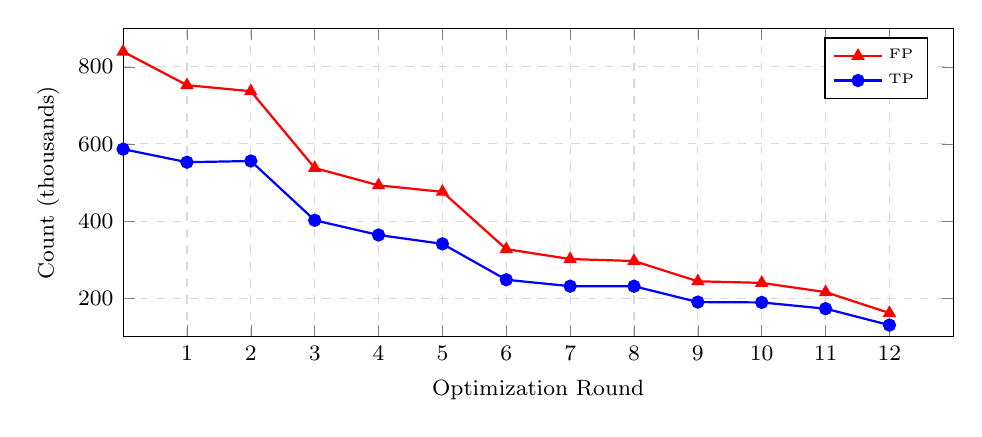
\begin{tikzpicture}
\begin{axis}[
    width=\columnwidth,
    height=5.5cm,
    xlabel={Optimization Round},
    ylabel={Count (thousands)},
    ymin=100, ymax=900,
    xmin=0, xmax=13,
    xtick={1,2,3,4,5,6,7,8,9,10,11,12},
    ylabel style={font=\footnotesize},
    xlabel style={font=\footnotesize},
    tick label style={font=\footnotesize},
    grid=major,
    grid style={dashed, gray!30},
    legend style={font=\tiny, at={(0.97,0.97)}, anchor=north east},
]
\addplot[color=red, mark=triangle*, thick] coordinates {
    (0, 839.3)
    (1, 752.4) (2, 736.6) (3, 537.6) (4, 492.6)
    (5, 475.8) (6, 327.2) (7, 301.5) (8, 296.4)
    (9, 243.8) (10, 239.7) (11, 215.7) (12, 161.5)
};
\addlegendentry{FP}
\addplot[color=blue, mark=*, thick] coordinates {
    (0, 586.5)
    (1, 552.6) (2, 555.7) (3, 402.0) (4, 363.9)
    (5, 340.9) (6, 247.8) (7, 231.1) (8, 231.0)
    (9, 189.9) (10, 189.0) (11, 172.8) (12, 130.2)
};
\addlegendentry{TP}
\end{axis}
\end{tikzpicture}
\caption{TP and FP counts across optimization rounds (full Juliet
suite, thousands).  Both decline as overly-broad rules are tightened;
the key metric is TP rate, which improved from 41.1\% to 44.6\%.}
\label{fig:fp-reduction}
\end{figure}

\subsection{The Header Problem}
\label{sec:fp-cross-file}

The first and largest source of false positives came from a fundamental
limitation of the tree-sitter approach: without \texttt{\#include}
resolution, every call to a function defined in another file looks like
a call to an undeclared function.  Rules DCL31-C and DCL07-C would flag
every \texttt{malloc()}, \texttt{printf()}, and \texttt{CreateFile()}
call.

The fix came in two stages.  First, a built-in database of standard
functions (Round 3, $-$198,974 FPs).  Second, cross-file analysis: a
pre-scan of project directories to discover all function definitions
(Round 6, $-$148,622 FPs).  Together, these two changes account for
41\% of the total FP reduction.

Later, adding $\sim$100 Windows API functions to the database
(Round 9) removed another 36K FPs from DCL31-C/DCL07-C alone---the
biggest single-rule win of any round.

\subsection{Type-Aware Analysis}

Several integer rules initially operated on the text of expressions
without considering the types of the operands.  This produced false
positives on non-integer types:

\begin{itemize}
    \item \texttt{char data; data + 1} was flagged as signed integer
        overflow (INT32-C).  Fix: \texttt{infer\_type()} returns
        ``not applicable'' for non-integer types.
    \item \texttt{ptr + n} was flagged as unsigned integer wrap
        (INT30-C).  Fix: pointer arithmetic is identified as valid C.
    \item Float-to-int assignments with unknown types were flagged
        (FLP34-C).  Fix: only flag when both sides have known,
        mismatched types.
\end{itemize}

The lesson: \emph{don't flag when uncertain.}  Suppressing warnings
for unknown or ambiguous types consistently improved the FP-to-TP
ratio.

\subsection{Bounds-Check Detection}

INT32-C and INT30-C gained AST-ancestor walking to detect enclosing
bounds checks.  The algorithm walks up to 15 ancestors looking for an
enclosing \texttt{if\_statement} whose condition references a type-limit
macro (\texttt{INT\_MAX}, \texttt{UINT64\_MAX}, etc.) \emph{and} at
least one arithmetic operand.

This achieved a 12.5:1 FP-to-TP reduction ratio for INT32-C.  One
important implementation detail: we use word-boundary matching for
macro names, because \texttt{ULONG\_MAX} contains \texttt{LONG\_MAX}
as a substring.

\subsection{Constant Evaluation}

The constant evaluator resolves $\sim$35 C standard limit macros,
$\sim$20 type sizes via \texttt{sizeof}, and arithmetic on these
values.  This produced the largest single-round FP reduction since
cross-file analysis ($-$12,088 FPs in Round 12), because it enabled
every integer rule to reason about allocation sizes, buffer bounds,
and guard conditions.

\subsection{Diminishing Returns}

\Cref{tab:fp-milestones} shows selected milestones.  The pattern of
diminishing returns is clear: Round 3 removed 199K FPs; by Round 8,
only 5K.  Each successive round requires more sophisticated analysis
for smaller gains.

\begin{table}[t]
\centering
\footnotesize
\begin{tabular}{@{}rlrrr@{}}
\toprule
\textbf{Rd} & \textbf{Key Change} & \textbf{FP} & \textbf{$\Delta$FP} & \textbf{TP\%} \\
\midrule
0 & Baseline (full suite) & 839K & --- & 41.1 \\
3 & Std function DB & 538K & $-$199K & 42.8 \\
6 & Cross-file analysis & 327K & $-$149K & 43.1 \\
9 & Windows API + types & 244K & $-$53K & 43.8 \\
12 & Const eval + macros & 162K & $-$12K & 44.6 \\
\midrule
\multicolumn{5}{@{}l}{\emph{Switch to fast-mode benchmarking (v0.3.20)}} \\
\midrule
--- & Fast-mode baseline & 24.7K & --- & 45.8 \\
--- & VRA + buffer analysis & 18.8K & $-$5.9K & 56.3 \\
--- & CFG const + CWE-369 & 17.0K & $-$1.8K & 60.2 \\
--- & Taint + return-value   & 14.1K & $-$2.9K & 63.6 \\
v0.3.119 & Precision improvements & 11.7K & $-$2.4K & 67.5 \\
v0.4.22 & VRA + STR31-C + EXP33-C & 9.9K & $-$1.8K & 72.7 \\
v0.4.46 & Opt-in INT provenance gating & 4.6K & $-$5.3K & 83.2 \\
v0.4.116 & Per-rule tuning (plateau) & 4.2K & $-$0.4K & 83.8 \\
\bottomrule
\end{tabular}
\caption{FP reduction milestones.  Full-suite rounds 0--12 reduced FP by
80.7\%.  Fast-mode continued from 45.8\% to 83.8\% TP rate.  The v0.4.22
row reflects continued VRA improvements, STR31-C buffer-size inference,
EXP33-C inter-procedural FP suppression, and crash-robustness fixes that
unlocked previously-aborted scans (raising both TP and FP).  v0.4.46
reflects the opt-in provenance-gated rewrite of INT30/31/32-C
(\cref{sec:provenance-frontier}), the single largest FP reduction since
cross-file analysis.  The 70 releases from v0.4.46 to v0.4.116 removed
only a further 0.4K FP (0.2 points of TP rate), the diminishing-returns
pattern continuing to its current extreme.}
\label{tab:fp-milestones}
\end{table}

\subsection{Principles That Emerged}

Five principles emerged from this iterative process:

\begin{enumerate}
    \item \textbf{Don't flag when uncertain.}  If the type, origin,
        or value of an operand is unknown, suppress the warning.
    \item \textbf{Target absolute FP counts, not rates.}  A rule with
        99\% FP rate and 100 violations matters less than one with
        50\% FP rate and 10K violations.
    \item \textbf{Zero-TP rules are free FP reductions.}  DCL40-C's
        31-character identifier prefix check produced 12K FPs and 0 TPs
        on Juliet.  Removing it was cost-free.
    \item \textbf{Verify on both benchmarks.}  Fixes targeting
        \texttt{uint32\_t} resolution show impact on real-world code
        but not on Juliet, which uses explicit C types.
    \item \textbf{Juliet is a rough approximation, not a proxy.}
        Treat the real-world suite as a first-class benchmark, run
        with the same rigor (versioned, committed, per-rule deltas
        reviewed) as Juliet.  Real-world code crashed the analyzer in
        ways Juliet structurally cannot (non-ASCII content,
        thousands-deep nesting, adversarial token ordering), exhibited
        per-rule regressions that Juliet scored as neutral or
        improved, and a sampled manual audit of the noisiest rules
        measured real-world precision far below what Juliet results
        implied.  Improvements validated only on Juliet have not, in
        our experience, earned the claim of working on real code.
\end{enumerate}

\subsection{The Residual Frontier: Provenance over Proof}
\label{sec:provenance-frontier}

The five principles above are all \emph{opt-out} refinements: each
suppresses a warning that sqc cannot prove dangerous.  A complete
file-at-a-time audit of SQLite---220 files at commit
\texttt{b1a73ba34d}, with every finding manually adjudicated---shows
where this philosophy reaches its limit.  INT32-C (signed integer
overflow) emitted 4{,}420 false positives against 15 true positives
(0.3\% precision), alone accounting for roughly one fifth of all of
sqc's false positives on the project.  Tracing the flagged source
lines is clarifying.  Every false positive is plain arithmetic on a
\emph{bounded} local integer---a register index (\texttt{regData-1}),
a statement counter (\texttt{db->nStatement-{}-}), a small loop count
(\texttt{nIdx+1}), a page-size sum (\texttt{szPage+szExtra}).  All 15
true positives involve an operand derived from \emph{untrusted,
unbounded} input: a varint decoded from a database blob, an
attacker-controlled cell count, a length read from a file, a value
parsed from the command line.  The discriminator is not the operation
but the \emph{provenance} of its operands.

This is not a value-range tuning problem.  sqc's VRA already proves
safety wherever a bound is visible; the residual false positives are
exactly the cases where the bound is a program invariant the analyzer
cannot see---a \texttt{SQLITE\_LIMIT} constant, an \texttt{assert}, a
data-structure size.  The bounded \texttt{nIdx+1} and the genuinely
dangerous \texttt{data+1} (where \texttt{data} came from
\texttt{atoi}) are \emph{syntactically identical}; only the origin of
the variable distinguishes them, so no amount of local proof closes
the gap.

The static-analysis literature splits cleanly on how to resolve this
(\cref{tab:optout-optin}).  Sound abstract-interpretation tools---%
Frama-C's Eva plugin~\cite{frama-c}, Infer's Inferbo buffer-overrun
domain~\cite{inferbo}, and CodeQL's range-analysis
library~\cite{codeql-range}---are \emph{opt-out}: they compute an
over-approximated (often \emph{symbolic}) interval for every variable
and emit an alarm unless they can prove the operation safe.  This
guarantees no false negatives but produces precisely the
bounded-counter alarms above; Inferbo's authors describe the outcome
as a deliberate ``balancing act'' and ship both a heuristic
post-filter and graded-confidence issue tiers
(\texttt{INTEGER\_OVERFLOW\_L1}\,$\ldots$\,\texttt{L5}, where the tier
encodes interval certainty and only the high-confidence tiers are on
by default).  Precision-oriented tools take the opposite stance.
ELAID~\cite{elaid}, the Clang Static Analyzer's taint
checker~\cite{clang-taint}, and INDIO~\cite{indio} are \emph{opt-in}:
an arithmetic operation becomes a candidate only when one of its
operands is tainted by untrusted input.  On ELAID's evaluation this
gate alone funnels away roughly 98\% of integer operations before any
overflow reasoning runs.

\begin{table}[t]
\centering
\footnotesize
\begin{tabular}{@{}lll@{}}
\toprule
\textbf{Model} & \textbf{Fires when} & \textbf{Representative tools} \\
\midrule
Opt-out & cannot prove safe & Eva, Inferbo, CodeQL \\
Opt-in  & operand is tainted & ELAID, Clang-taint, INDIO \\
\bottomrule
\end{tabular}
\caption{Two design philosophies for integer-overflow reporting.
sqc's INT rules were re-implemented from opt-out to opt-in provenance
gating, eliminating about 93\% of the residual SQLite false positives.}
\label{tab:optout-optin}
\end{table}

sqc's INT rules were originally opt-out, which put them in direct
tension with our own first principle---\emph{don't flag when
uncertain}---for the bounded-counter case, where uncertainty about a
variable's bound was silently treated as risk.  We therefore
re-implemented INT30-C, INT31-C, and INT32-C as \emph{opt-in}
provenance gates.  Unlike the IO2BO checkers above, a general
INT30/31/32-C rule has no single allocation \emph{sink} to gate on;
for sqc the arithmetic operation (or lossy conversion) is itself the
sink, so the gate reduces to ``does any operand derive from untrusted
or unbounded input.''  An operand is treated as risky when it flows
from a recognized source---a full-range parser (\texttt{atoi},
\texttt{strtol}, \texttt{rand}), an environment/IO taint source, an
untrusted-decode accessor (varint readers, \texttt{ftell}), a
tainted-summary callee return reused from sqc's cross-function
summaries (\cref{sec:prescan}), or a tainted global---or when VRA
proves the expression \emph{definitely} overflows (every value in the
computed range is out of bounds, e.g.\ \texttt{INT\_MAX+1}); operands
with merely unknown-but-bounded ranges are suppressed.

The effect on real-world precision is large.  On the full SQLite
census (\cref{sec:realworld-results}), the gate eliminates 91.8\% of INT32-C,
98.9\% of INT30-C, and 96.9\% of INT31-C false positives---about 93\%
of the roughly 5{,}750 adjudicated INT false positives overall---while
INT31-C retains all three of its true positives and INT32-C retains
eight of fifteen.  The cost is recall, and it is real: on Juliet the
INT detection rate falls to 45--50\% (from near-complete), because
opt-in gating misses an overflow whenever the tainted operand reaches
the sink across a function boundary that sqc's summaries do not
propagate---the dominant residual gap.  This is the precision/recall
tradeoff made concrete: the synthetic suite, built so that every
flagged operation is genuinely reachable, rewards the opt-out policy
that the real-world census punishes.  We regard the exchange as
favorable for deployment---thousands of false alarms removed per
project against a recall reduction confined to inter-procedural flows
that a fielded tool can recover through targeted source annotations,
and we validated it on both benchmarks before adopting it.

A coda illustrates the audit's value independent of sqc's rule set.
While adjudicating the 220-file SQLite census, manual review of
\texttt{os\_kv.c} found a heap buffer overflow in
\texttt{kvvfsDecode()}: its hex-pair decoding branch writes to
\texttt{aOut[j]} with no bounds check, while the adjacent zero-run
branch in the same function already guards with \texttt{if(j+n>nOut)
return -1;}---a journal record with a short length header followed by
a long run of hex pairs overflows the destination buffer.  sqc does
not flag this site; the unguarded write is not an arithmetic operation
any INT or ARR rule's provenance gate fires on, so it is a false
negative for the tool, not a suppressed true positive.  We reported it
upstream\footnote{\url{https://sqlite.org/bugs/forumpost/afbc56be7b}},
and the SQLite team confirmed and fixed it the same day (check-in
\texttt{732c8f81b5a91483}).  The finding did not come from sqc's
output, but from the close reading sqc's findings prompted---evidence
that the audit methodology, not just the rule set, is part of what the
tool delivers, and a concrete direction for a new rule: an unguarded
write alongside a bounds-checked sibling branch in the same function.

The complementary case came directly from the rule set.  sqc's INT32-C
provenance gate flagged \texttt{fts5SegmentSize()} in
\texttt{ext/fts5/fts5\_index.c}: \texttt{1 + pSeg->pgnoLast -
pSeg->pgnoFirst}, where both fields are decoded straight from an
on-disk \texttt{\%\_data} shadow-table structure record via
\texttt{fts5GetVarint32()}.  The only validation on decode is
\texttt{pgnoLast < pgnoFirst}, which rejects an out-of-order pair but
places no upper bound on \texttt{pgnoLast} itself, so a crafted or
corrupted structure record can drive the subtraction to a signed
integer overflow (\texttt{pgnoFirst = 0}, \texttt{pgnoLast = INT\_MAX}
reproduces it under UBSan).  Adjudication during the 220-file census
confirmed this as a genuine true positive rather than a suppressed
false alarm.  We reported it
upstream\footnote{\url{https://sqlite.org/bugs/info/2026-08-17T20:07:33Z}},
and it was likewise fixed the same day (check-in
\texttt{c97a940ceb}).  Unlike the kvvfsDecode finding above, this one
is squarely inside what the rule set is designed to catch---an
untrusted-provenance operand reaching an unguarded arithmetic
sink---and its same-day confirmation and fix is direct external
validation of an opt-in INT32-C true positive, not just of the audit
process that surrounds the tool.
